\begin{frame}
  \frametitle{Protocol Design Considerations}
     \uncover<1->{  Design considerations:}
  \begin{enumerate}
     \uncover<2->{  \item Graph workloads exhibit high contention}
     \uncover<3->{  \item Graph transactions tend to be longer-lived than those in other databases}
  \end{enumerate}
     \uncover<4->{\textbf{Protocol must permit multiple updates on the same distributed edge provided they are \textit{sufficiently} apart in time to ensure reciprocal consistency}}
\end{frame}

\begin{frame}
  \frametitle{\tDelta Protocol}
  \begin{itemize}
  \uncover<1->{  \item \textbf{Fact:} a transaction updating a distributed edge must update one edge pointer then \textbf{immediately} update the other}
  \uncover<2->{  \item \textbf{Rule:} an update is permitted if the immediately preceding update was done at least $\Delta$ time before. Else, abort}
  \uncover<3->{  \item \textbf{Assumption:} the time interval that elapses between completing an update at one edge pointer and starting at the other can be estimated to be $\delta$.}
    \uncover<4->{ \item \textbf{Parameter Selection:} Choose $\Delta > \delta$}
  \end{itemize}
\end{frame}

\begin{frame}
  \frametitle{\tDelta Protocol: Example}
  \begin{center}
    \textbf{\small{Rule: an update is permitted if the preceding update was done at least $\Delta$ time before. Else, abort}}
  \end{center}
  \begin{figure}[h!]
    \centering
    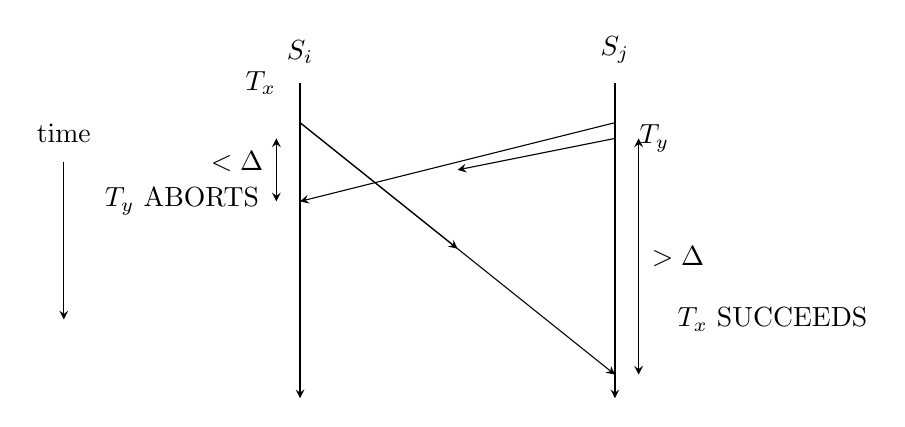
\begin{tikzpicture}
      \uncover<2->{
        \draw [black,<-,>=stealth] (-3,1) -- (-3,3) node [label=above:{time}] {};
        \draw [black,<-,>=stealth] (0,0) -- (0,4) node [label=above:{$S_i$}] {};
        \draw [black,<-,>=stealth] (4,0) -- (4,4)  node [label=above:{$S_j$}] {};
              \draw [white,<-,>=stealth] (7,1) -- (7,3) ;
      }
      \uncover<2->{
        \node [] at (-0.5,4) {$T_x$};
      }
      \uncover<3-6>{
        \draw [->,>=stealth] (0,3.5) -- (2,1.9);
      }
      \uncover<4->{
        \node [] at (4.5,3.3) {$T_y$};
      }
      \uncover<5-5>{
        \draw [->,>=stealth] (4,3.3) -- (2,2.9);
      }
      \uncover<6-8>{
        \draw [->,>=stealth] (4,3.5) -- (0,2.5);
      }
      \uncover<6-8>{
        \draw [<->,>=stealth] (-0.3,2.5) -- (-0.3,3.3);
        \node[] at (-0.8,3) {$< \Delta$};
        \node[] at (-1.5,2.5) {$T_y$ ABORTS};
      }
      \uncover<7->{
        \draw [->,>=stealth] (0,3.5)  -- (4,0.3);
      }
      \uncover<8-8>{
        \node[] at (6,1) {$T_x$ SUCCEEDS};
        \draw [<->,>=stealth] (4.3,0.3) -- (4.3,3.3);
        \node[] at (4.8,1.8) {$> \Delta$};
      }
    \end{tikzpicture}
  \end{figure}
\end{frame}

\begin{frame}
  \frametitle{\tDelta Protocol}
  \begin{itemize}
    \uncover<1->{  \item Reciprocal consistency is preserved if the time taken to complete an update at one edge pointer and start at other remains less than $\Delta$}
    \uncover<2->{  \item If $\Delta$ is exceeded then reciprocal inconsistency and hence semantic corruption can occur}
      \uncover<3->{  \item Setting a large $\Delta$ tends to preserve consistency but leads to more aborted transactions}
  \end{itemize}
\end{frame}